\chapter{Use of AI}
The detailed prompt of the use of ChatGPT 4o \autocite{gpt-websocket} is as in Figure \ref{fig:gpt-websocket-1}, Figure \ref{fig:gpt-websocket-2} and Figure \ref{fig:gpt-websocket-3}. For the ease of reference, the code is also included in \ref{code-listing:gpt-websocket}.

\begin{figure}[htp]
    \centering

    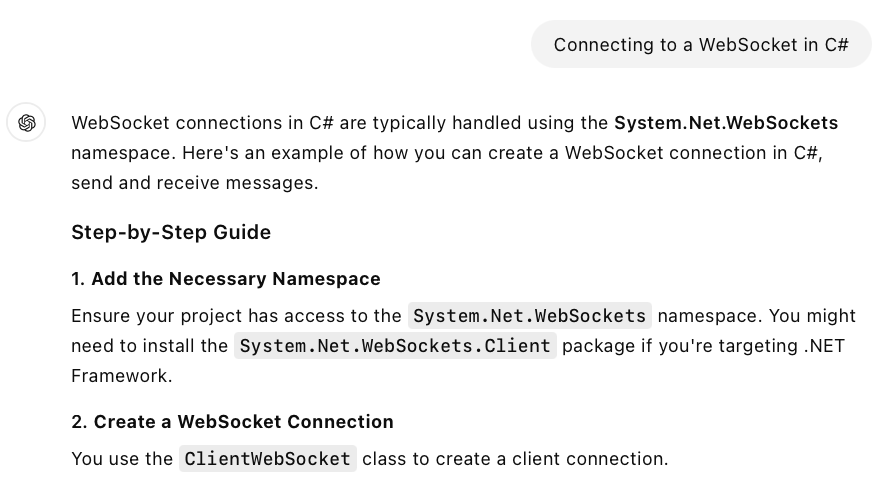
\includegraphics[width=0.8\linewidth]{gpt-p1.png}
    \caption[Prompt to ChatGPT in \autocite{gpt-websocket}, Part 1]{Prompt to ChatGPT in \autocite{gpt-websocket}, Part 1}
    \label{fig:gpt-websocket-1}
\end{figure}

\begin{figure}[htp]
    \centering

    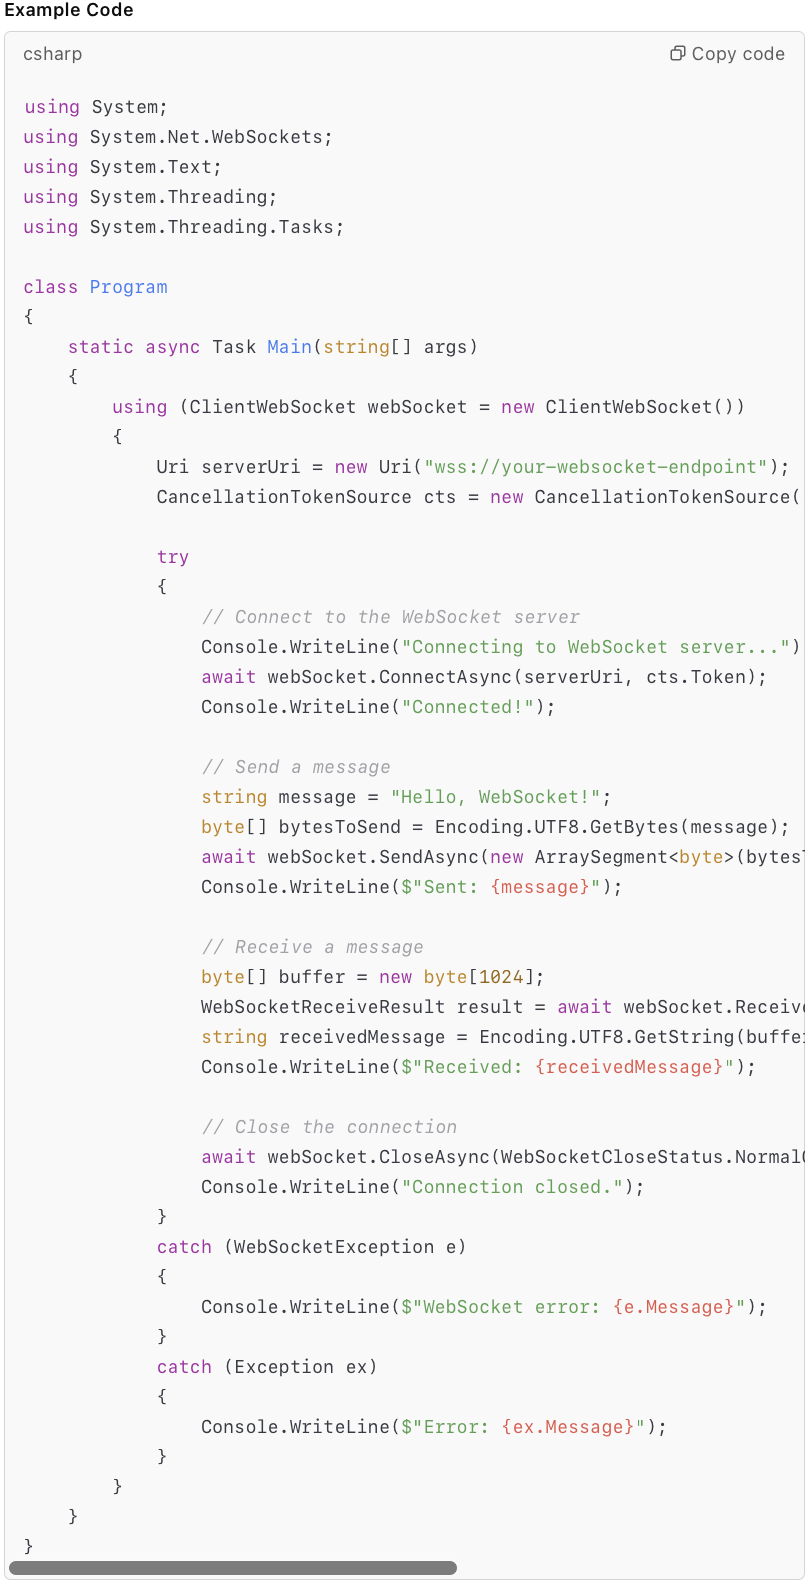
\includegraphics[width=0.45\linewidth]{gpt-c1.png}
    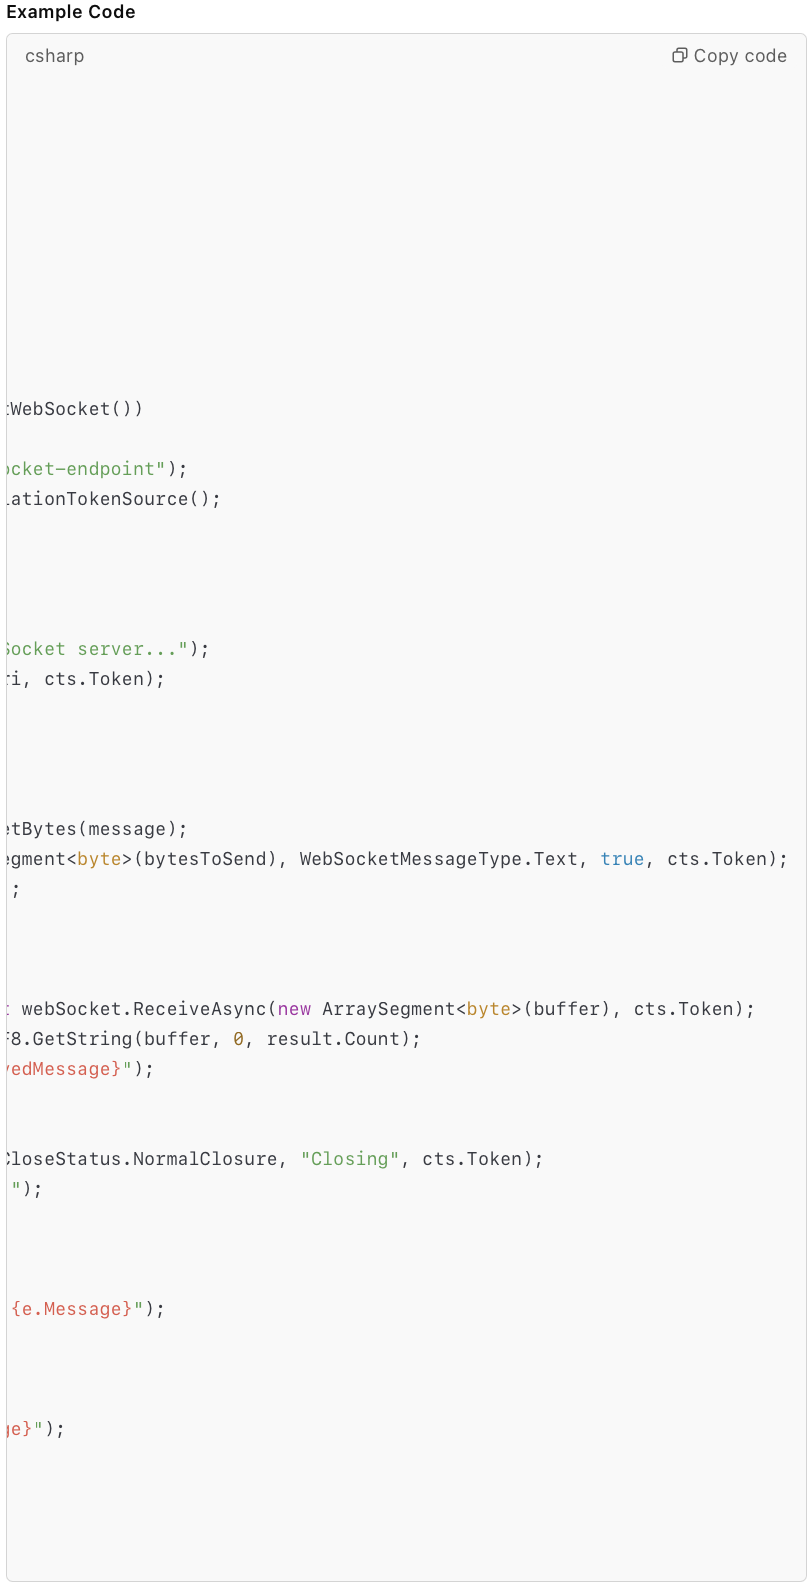
\includegraphics[width=0.45\linewidth]{gpt-c2.png}

    \caption[Prompt to ChatGPT in \autocite{gpt-websocket}, Part 2]{Prompt to ChatGPT in \autocite{gpt-websocket}, Part 2}
    \label{fig:gpt-websocket-2}
\end{figure}

\begin{figure}[htp]
    \centering

    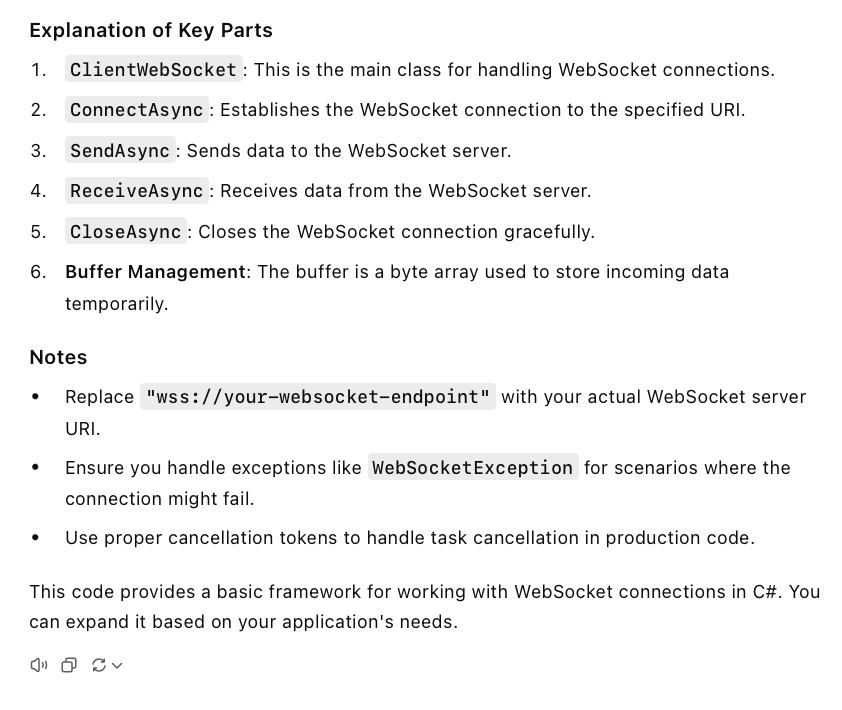
\includegraphics[width=0.8\linewidth]{gpt-p2.png}

    \caption[Prompt to ChatGPT in \autocite{gpt-websocket}, Part 3]{Prompt to ChatGPT in \autocite{gpt-websocket}, Part 3}
    \label{fig:gpt-websocket-3}
\end{figure}

This is used to outline a working example of \Code{System.Net.WebSocket} class and the author made numerous edits and additions to eventually create commit \Code{8f8f6e9} on the same day, and other references such as StackOverflow \autocite{stackoverflow-websocket-demo, stackoverflow-websocket-demo-2} and the official Microsoft Documentation \autocite{dotnet-reference-clientwebsocket} has also been used to create the relevant code in WebSocket connections.

This code has eventually been refactored and removed in \Code{60b660a}, still referencing the sources \autocite{stackoverflow-websocket-demo, stackoverflow-websocket-demo-2}.